%%% Title:    Missing Data Stats Camp Course: FIML
%%% Author:   Kyle M. Lang
%%% Created:  < 2015-SEP-29
%%% Modified: 2018-OCT-19

\documentclass{beamer}\usepackage[]{graphicx}\usepackage[]{color}
%% maxwidth is the original width if it is less than linewidth
%% otherwise use linewidth (to make sure the graphics do not exceed the margin)
\makeatletter
\def\maxwidth{ %
  \ifdim\Gin@nat@width>\linewidth
    \linewidth
  \else
    \Gin@nat@width
  \fi
}
\makeatother

\definecolor{fgcolor}{rgb}{0, 0, 0}
\newcommand{\hlnum}[1]{\textcolor[rgb]{0.69,0.494,0}{#1}}%
\newcommand{\hlstr}[1]{\textcolor[rgb]{0.749,0.012,0.012}{#1}}%
\newcommand{\hlcom}[1]{\textcolor[rgb]{0.514,0.506,0.514}{\textit{#1}}}%
\newcommand{\hlopt}[1]{\textcolor[rgb]{0,0,0}{#1}}%
\newcommand{\hlstd}[1]{\textcolor[rgb]{0,0,0}{#1}}%
\newcommand{\hlkwa}[1]{\textcolor[rgb]{0,0,0}{\textbf{#1}}}%
\newcommand{\hlkwb}[1]{\textcolor[rgb]{0,0.341,0.682}{#1}}%
\newcommand{\hlkwc}[1]{\textcolor[rgb]{0,0,0}{\textbf{#1}}}%
\newcommand{\hlkwd}[1]{\textcolor[rgb]{0.004,0.004,0.506}{#1}}%
\let\hlipl\hlkwb

\usepackage{framed}
\makeatletter
\newenvironment{kframe}{%
 \def\at@end@of@kframe{}%
 \ifinner\ifhmode%
  \def\at@end@of@kframe{\end{minipage}}%
  \begin{minipage}{\columnwidth}%
 \fi\fi%
 \def\FrameCommand##1{\hskip\@totalleftmargin \hskip-\fboxsep
 \colorbox{shadecolor}{##1}\hskip-\fboxsep
     % There is no \\@totalrightmargin, so:
     \hskip-\linewidth \hskip-\@totalleftmargin \hskip\columnwidth}%
 \MakeFramed {\advance\hsize-\width
   \@totalleftmargin\z@ \linewidth\hsize
   \@setminipage}}%
 {\par\unskip\endMakeFramed%
 \at@end@of@kframe}
\makeatother

\definecolor{shadecolor}{rgb}{.97, .97, .97}
\definecolor{messagecolor}{rgb}{0, 0, 0}
\definecolor{warningcolor}{rgb}{1, 0, 1}
\definecolor{errorcolor}{rgb}{1, 0, 0}
\newenvironment{knitrout}{}{} % an empty environment to be redefined in TeX

\usepackage{alltt}
\usetheme[%
  pageofpages          = of,
  bullet               = circle,
  titleline            = true,
  alternativetitlepage = true,
  titlepagelogo        = Logo3,
  watermark            = watermarkTiU,
  watermarkheight      = 100px,
  watermarkheightmult  = 4%
]{UVT}

\usepackage{graphicx}
\usepackage{booktabs}
\usepackage[natbibapa]{apacite}
\usepackage[libertine]{newtxmath}
\usepackage{fancybox}
\usepackage[mathcal]{eucal}
\usepackage{upgreek}
\usepackage{caption}

\newcommand{\kfold}[0]{\emph{K}-fold cross-validation}
\newcommand{\mub}[0]{\boldsymbol{\muup}}

%% Ensure styles of `blocks' (used in Definitions, Theorems etc.) follows the
%% UVT-style theme:
\setbeamercolor{block title}{fg = darkblue, bg = white}
\setbeamercolor{block body}{use = block title, bg = block title.bg}

%% Ensure TableOfContents is in UVT-style theme:
\setbeamercolor{section in toc}{fg = darkblue}

%% Don't label table captions:
\captionsetup{labelformat = empty}

\title{Full Information Maximum Likelihood}
\subtitle{Stats Camp 2018: Missing Data Analysis}
\author{Kyle M. Lang}
\institute{Department of Methodology \& Statistics\\Tilburg University}
\date{19--21 October 2018}
\IfFileExists{upquote.sty}{\usepackage{upquote}}{}
\begin{document}

%------------------------------------------------------------------------------%



%------------------------------------------------------------------------------%

\begin{frame}[t,plain]

  \titlepage

\end{frame}

%------------------------------------------------------------------------------%

\begin{frame}{Outline}

  \begin{itemize}
  \item Look at FIML in more depth
    \va
    \begin{itemize}
    \item Review of maximum likelihood (ML)
    \item Show how to do ML and FIML manually in \textsf{R}.
    \end{itemize}
  \end{itemize}
    
\end{frame}

%------------------------------------------------------------------------------%

\begin{frame}{FIML Conceptual Refresher}

  FIML is an ML estimation method that is robust to ignorable nonresponse.
  \vc
  \begin{itemize}
  \item FIML partitions the missing information out of the likelihood function 
    so that the model is only estimated from the observed parts of the data.
  \end{itemize}
  \vb
  After a minor alteration to the likelihood function, FIML reduces to simple ML 
  estimation.
  \vc
  \begin{itemize}
  \item So, let's review ML estimation before moving forward.
  \end{itemize}
  
\end{frame}

%------------------------------------------------------------------------------%

\begin{frame}[allowframebreaks]{Maximum Likelihood Estimation Refresher}

  ML estimation simply finds the parameter values that are ``most likely'' to 
  have given rise to the observed data.
  \vb
  \begin{itemize}
  \item The \emph{likelihood} function is just a probability density (or mass) 
    function with the data treated as fixed and the parameters treated as 
    random variables.
    \vb
  \item Having such a framework allows us to ask: ``Given that I've observed 
    these data values, what parameter values most probably describe these 
    data?''
  \end{itemize}
  
  \pagebreak
  
  ML estimation is usually employed when there is no closed form solution for 
  the parameters we seek.
  \vb
  \begin{itemize}
  \item This is why you don't usually see ML used to fit general linear models.
  \end{itemize}
  \vb
  After choosing a likelihood function, we iteratively optimize the function to 
  produce the ML estimated parameters.
  \vb
  \begin{itemize}
  \item In practice, we nearly always work with the natural logarithm of the 
    likelihood function (i.e., the \emph{loglikelihood}).
  \end{itemize}
  
\end{frame}

\watermarkoff %----------------------------------------------------------------%

\begin{frame}{Likelihoods}
  
  \begin{columns}
    \begin{column}{0.5\textwidth}
      
      Suppose we have the following model:
      \begin{align*}
        Y \sim \text{N}\left( \mu, \sigma^2 \right).
      \end{align*}
      
    \end{column}
    \begin{column}{0.5\textwidth}
      
\begin{knitrout}\footnotesize
\definecolor{shadecolor}{rgb}{0.878, 0.918, 0.933}\color{fgcolor}

{\centering 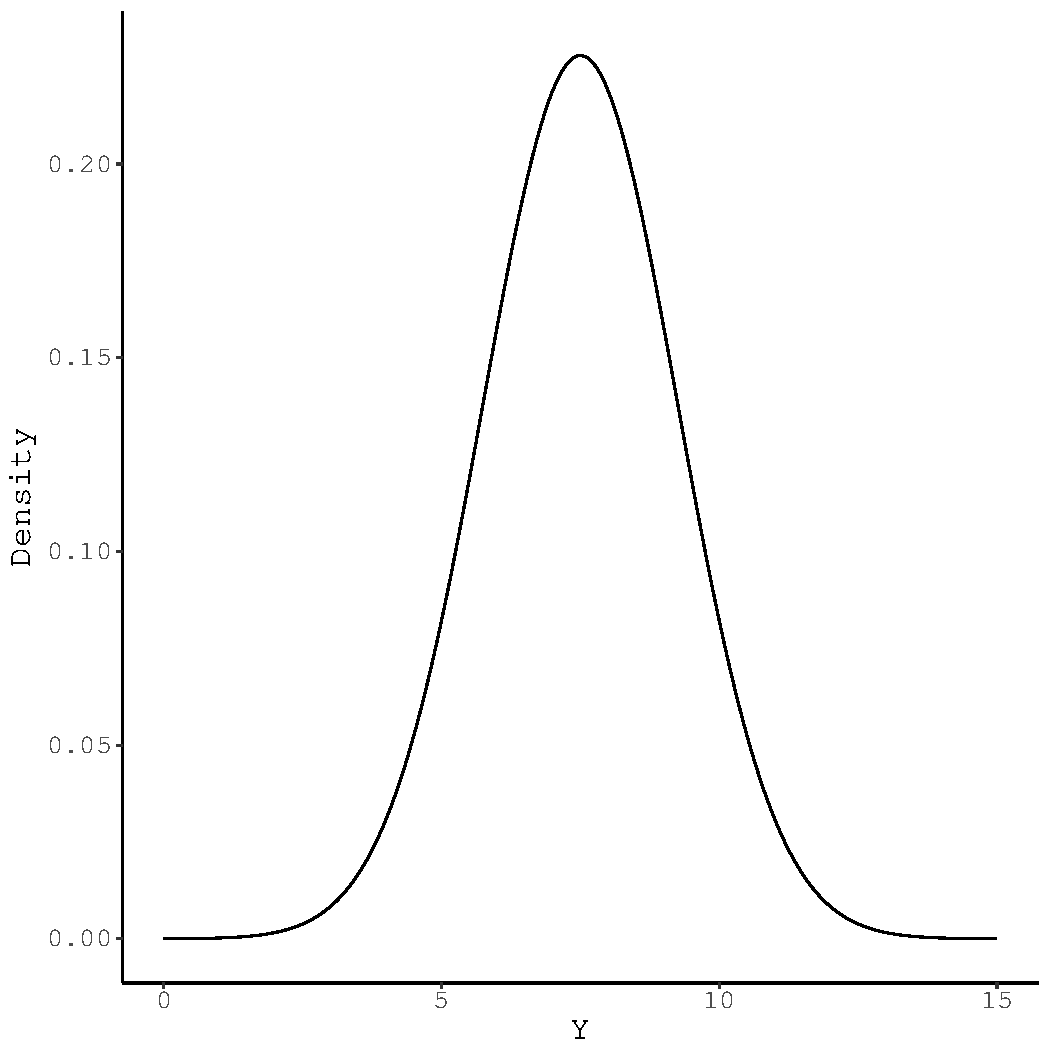
\includegraphics[width=\maxwidth]{figure/unnamed-chunk-1-1} 

}



\end{knitrout}

\end{column}
\end{columns}

\end{frame}

\watermarkon %-----------------------------------------------------------------%

\begin{frame}{Likelihoods}
  
  For a given $Y_n$, we have:
  \begin{align}
    P \left( Y_n|\mu, \sigma^2 \right) = 
    \frac{1}{\sqrt{2 \pi \sigma^2}} 
    e^{-\frac{\left( Y_n - \mu \right)^2}{2\sigma^2}}. \label{margPdf}
  \end{align}
  
  If we plug estimated parameters into Equation \ref{margPdf}, we get the 
  probability of observing $Y_n$ given $\hat{\mu}$ and $\hat{\sigma}^2$:
  \begin{align}
    P \left( Y_n|\hat{\mu}, \hat{\sigma}^2 \right) = 
    \frac{1}{\sqrt{2 \pi \hat{\sigma}^2}} 
    e^{-\frac{\left( Y_n - \hat{\mu}\right)^2}{2\hat{\sigma}^2}}. \label{estMargPdf}
  \end{align}
  
  Applying Equation \ref{estMargPdf} to all $N$ observations and multiplying the 
  results produces a \emph{likelihood}:
  \begin{align*}
    \hat{L} \left( \hat{\mu}, \hat{\sigma}^2 \right) = 
    \prod_{n = 1}^N P \left( Y_n|\hat{\mu}, \hat{\sigma}^2 \right).
  \end{align*}
  
\end{frame}

%%----------------------------------------------------------------------------%%

\begin{frame}{Likelihoods}
  
  We generally want to work with the natural logarithm of Equation 
  \ref{estMargPdf}. Doing so gives the \emph{loglikelihood}:
  \begin{align*}
  \hat{\mathcal{L}} \left( \hat{\mu}, \hat{\sigma}^2 \right) &= 
    \ln \prod_{n = 1}^N P \left( Y_n|\hat{\mu}, \hat{\sigma}^2 \right)\\ 
    &= -\frac{N}{2} \ln 2\pi - N \ln \hat{\sigma} - \frac{1}{2\hat{\sigma}^2} 
    \sum_{n = 1}^N \left( Y_n - \hat{\mu} \right)^2
  \end{align*}
  
  ML tries to find the values of $\hat{\mu}$ and $\hat{\sigma}^2$ that maximize 
  $\hat{\mathcal{L}} \left( \hat{\mu}, \hat{\sigma}^2 \right)$.
  \vc
  \begin{itemize}
  \item Find the values of $\hat{\mu}$ and $\hat{\sigma}^2$ that are \emph{most 
    likely}, given the observed values of $Y$.
  \end{itemize}
  
\end{frame}

\watermarkoff %----------------------------------------------------------------%

\begin{frame}{Likelihoods}
  
    \begin{columns}
    \begin{column}{0.5\textwidth}
      
      Suppose we have a linear regression model:
      \begin{align*}
        Y &= \beta_0 + \beta_1 X + \varepsilon,\\[6pt]
        \varepsilon &\sim \text{N}\left( 0, \sigma^2 \right).
      \end{align*}
      This model can be equivalently written as:
      \begin{align*}
        Y \sim \text{N} \left( \beta_0 + \beta_1 X, \sigma^2 \right)
      \end{align*}
      
    \end{column}
    \begin{column}{0.5\textwidth}

      \begin{figure}
        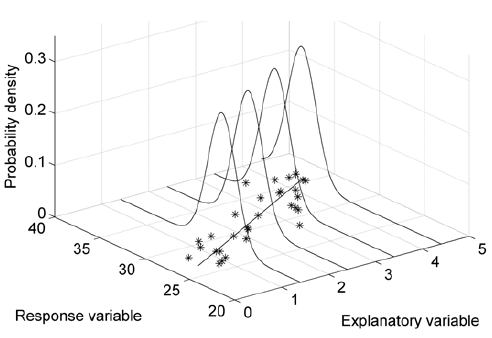
\includegraphics[width = \textwidth]{figures/conditional_density_figure.png}\\
        \va
        \tiny{Image retrieved from:
          \url{http://www.seaturtle.org/mtn/archives/mtn122/mtn122p1.shtml}}
      \end{figure}
      
    \end{column}
    \end{columns}
    
\end{frame}

\watermarkon %-----------------------------------------------------------------%

\begin{frame}{Likelihoods}
  
  For a given $\{Y_n, X_n\}$, we have:
  \begin{align}
    P \left( Y_n|X_n, \beta_0, \beta_1, \sigma^2 \right) = 
    \frac{1}{\sqrt{2 \pi \sigma^2}} 
    e^{-\frac{\left( Y_n - \beta_0 - \beta_1 X_n \right)^2}{2\sigma^2}}. \label{olsPdf}
  \end{align}
  
  If we plug our estimated parameters into Equation \ref{olsPdf}, we get the 
  probability of observing $Y_n$ given $\hat{Y}_n = \hat{\beta}_0 + 
  \hat{\beta}_1X_n$ and $\hat{\sigma}^2$.
  \begin{align}
    P \left( Y_n|X_n, \hat{\beta}_0, \hat{\beta}_1, \hat{\sigma}^2 \right) = 
    \frac{1}{\sqrt{2 \pi \hat{\sigma}^2}} 
    e^{-\frac{\left( Y_n - \hat{\beta}_0 - \hat{\beta}_1 X_n \right)^2}{2\hat{\sigma}^2}} \label{estOlsPdf}
  \end{align}
  
\end{frame}

%------------------------------------------------------------------------------%

\begin{frame}{Likelihoods}
 
  So, our final loglikelihood function would be the following:
  \begin{align*}
  \hat{\mathcal{L}} \left( \hat{\beta}_0, \hat{\beta}_1, \hat{\sigma}^2 \right) &= 
    \ln \prod_{n = 1}^N P \left( Y_n|X_n, \hat{\beta}_0, \hat{\beta}_1, \hat{\sigma}^2 \right)\\ 
    &= -\frac{N}{2} \ln 2\pi - N \ln \hat{\sigma} - \frac{1}{2\hat{\sigma}^2} 
    \sum_{n = 1}^N \left( Y_n - \hat{\beta}_0 - \hat{\beta}_1 X_n \right)^2.
  \end{align*}
  
\end{frame}
  
\watermarkoff %----------------------------------------------------------------%

\begin{frame}[fragile, allowframebreaks]{Example}
    


\begin{knitrout}\footnotesize
\definecolor{shadecolor}{rgb}{0.878, 0.918, 0.933}\color{fgcolor}\begin{kframe}
\begin{alltt}
\hlcom{## Fit a model:}
\hlstd{out1} \hlkwb{<-} \hlkwd{lm}\hlstd{(ldl} \hlopt{~} \hlstd{bp} \hlopt{+} \hlstd{glu} \hlopt{+} \hlstd{bmi,} \hlkwc{data} \hlstd{= diabetes)}

\hlcom{## Extract the predicted values and estimated residual }
\hlcom{## standard error:}
\hlstd{yHat} \hlkwb{<-} \hlkwd{predict}\hlstd{(out1)}
\hlstd{s}    \hlkwb{<-} \hlkwd{summary}\hlstd{(out1)}\hlopt{$}\hlstd{sigma}

\hlcom{## Compute the row-wise probabilities:}
\hlstd{pY} \hlkwb{<-} \hlkwd{dnorm}\hlstd{(diabetes}\hlopt{$}\hlstd{ldl,} \hlkwc{mean} \hlstd{= yHat,} \hlkwc{sd} \hlstd{= s)}

\hlcom{## Compute the loglikelihood, and compare to R's version:}
\hlkwd{sum}\hlstd{(}\hlkwd{log}\hlstd{(pY));} \hlkwd{logLik}\hlstd{(out1)[}\hlnum{1}\hlstd{]}
\end{alltt}
\begin{verbatim}
## [1] -2109.939
## [1] -2109.93
\end{verbatim}
\end{kframe}
\end{knitrout}

\end{frame}

\watermarkon %-----------------------------------------------------------------%

\begin{frame}{Multivariate Normal Distribution}
  
  The PDF for the multivariate normal distribution is:
  \begin{align*}
    P(\mathbf{Y}|\mub, \Sigma) = 
    \frac{1}{\sqrt{(2\pi)^P|\Sigma|}} e^{-\frac{1}{2}(\mathbf{Y} - \mub)^T\Sigma^{-1}(\mathbf{Y} - \mub)}.
  \end{align*}
  So, the multivariate normal loglikelihood is:
  \begin{align*}
    \mathcal{L} \left( \mub, \Sigma \right) = 
    -\left[\frac{P}{2} \ln(2\pi) + \frac{1}{2} \ln |\Sigma| + \frac{1}{2} \right] \sum_{n = 1}^N(\mathbf{Y}_n - \mub)^T \Sigma^{-1}(\mathbf{Y}_n - \mub).
  \end{align*}
  Which can be further simplified if we multiply through by -2:
  \begin{align*}
    -2\mathcal{L} \left( \mub, \Sigma \right) = 
    \left[P \ln(2\pi) + \ln |\Sigma| \right] \sum_{n = 1}^N(\mathbf{Y}_n - \mub)^T \Sigma^{-1}(\mathbf{Y}_n - \mub).
  \end{align*}
  
\end{frame}

%%----------------------------------------------------------------------------%%

\begin{frame}{Steps of ML}

  \begin{enumerate}
  \item Choose a probability distribution, $f(Y|\theta)$, to describe the 
    distribution of the data, $Y$, given the parameters, $\theta$.
    \vc
  \item Choose some estimate of $\theta$, $\hat{\theta}^{(i)}$.
    \vc
  \item Compute each row's contribution to the loglikelihood function by 
    evaluating: $\ln \left[f\left(Y_n|\hat{\theta}^{(i)}\right)\right]$. 
    \label{rowContrib}
    \vc
  \item Sum the individual loglikelihood contributions from Step 
    \ref{rowContrib} to find the loglikelihood value, $\hat{\mathcal{L}}$. 
    \label{getLL}
    \vc
  \item Choose a ``better'' estimate of the parameters, $\hat{\theta}^{(i + 1)}$, 
    and repeat Steps \ref{rowContrib} and \ref{getLL}. \label{updateTheta}
    \vc
  \item Repeat Steps \ref{rowContrib} -- \ref{updateTheta} until the change 
    between $LL^{(i - 1)}$ and $LL^{(i)}$ falls below some trivially small 
    threshold.
    \vc
  \item Take $\hat{\theta}^{(i)}$ as your estimated parameters.
  \end{enumerate}

\end{frame}

\watermarkoff %----------------------------------------------------------------%

\begin{frame}[fragile]{ML Example}
  
  Recall the $n$th observation's contribution to the multivariate normal 
  loglikelihood function:
  \begin{align*}
   \mathcal{L} \left( \mub, \Sigma \right)_n = 
   -\frac{P}{2} \ln(2\pi) - \frac{1}{2} \ln |\Sigma| - \frac{1}{2} (\mathbf{Y}_n - \mub)^T \Sigma^{-1}(\mathbf{Y}_n - \mub).
  \end{align*}

  \va

  It turns out that this function is readily available in R via the 
  \textbf{mvtnorm} package:

\begin{knitrout}\footnotesize
\definecolor{shadecolor}{rgb}{0.878, 0.918, 0.933}\color{fgcolor}\begin{kframe}
\begin{alltt}
\hlcom{## Vector of row-wise contributions to the overall LL:}
\hlstd{ll0} \hlkwb{<-} \hlkwd{dmvnorm}\hlstd{(y,} \hlkwc{mean} \hlstd{= mu,} \hlkwc{sigma} \hlstd{= sigma,} \hlkwc{log} \hlstd{=} \hlnum{TRUE}\hlstd{)}
\end{alltt}
\end{kframe}
\end{knitrout}

\end{frame}

%------------------------------------------------------------------------------%

\begin{frame}[fragile]{ML Example}

  We can wrap the preceding code in a nice \textsf{R} function:

\begin{knitrout}\footnotesize
\definecolor{shadecolor}{rgb}{0.878, 0.918, 0.933}\color{fgcolor}\begin{kframe}
\begin{alltt}
\hlcom{## Complete data loglikelihood function:}
\hlstd{ll} \hlkwb{<-} \hlkwa{function}\hlstd{(}\hlkwc{par}\hlstd{,} \hlkwc{data}\hlstd{) \{}
    \hlcom{## Extract the parameter matrices:}
    \hlstd{p}  \hlkwb{<-} \hlkwd{ncol}\hlstd{(data)}
    \hlstd{mu} \hlkwb{<-} \hlstd{par[}\hlnum{1} \hlopt{:} \hlstd{p]}

    \hlcom{## Populate sigma from its Cholesky factor:}
    \hlstd{sigma} \hlkwb{<-}\hlkwd{vecChol}\hlstd{(par[}\hlopt{-}\hlkwd{c}\hlstd{(}\hlnum{1} \hlopt{:} \hlstd{p)],} \hlkwc{revert} \hlstd{=} \hlnum{TRUE}\hlstd{)}

    \hlcom{## Compute the row-wise contributions to the LL:}
    \hlstd{ll0} \hlkwb{<-}
        \hlkwd{dmvnorm}\hlstd{(data,} \hlkwc{mean} \hlstd{= mu,} \hlkwc{sigma} \hlstd{= sigma,} \hlkwc{log} \hlstd{=} \hlnum{TRUE}\hlstd{)}

    \hlkwd{sum}\hlstd{(ll0)}\hlcom{# return the overall LL value}
\hlstd{\}}
\end{alltt}
\end{kframe}
\end{knitrout}

\end{frame}

%------------------------------------------------------------------------------%

\begin{frame}[fragile]{ML Example}

  We'll also need the helper functions:
  
\begin{knitrout}\footnotesize
\definecolor{shadecolor}{rgb}{0.878, 0.918, 0.933}\color{fgcolor}\begin{kframe}
\begin{alltt}
\hlcom{## Convert from covariance matrix to vectorized Cholesky }
\hlcom{## factor and back:}
\hlstd{vecChol} \hlkwb{<-} \hlkwa{function}\hlstd{(}\hlkwc{x}\hlstd{,} \hlkwc{revert} \hlstd{=} \hlnum{FALSE}\hlstd{) \{}
    \hlkwa{if}\hlstd{(revert) \{}
        \hlstd{tmp}                  \hlkwb{<-} \hlkwd{matrix}\hlstd{(}\hlnum{0}\hlstd{,} \hlkwd{nV}\hlstd{(x),} \hlkwd{nV}\hlstd{(x))}
        \hlstd{tmp[}\hlopt{!}\hlkwd{lower.tri}\hlstd{(tmp)]} \hlkwb{<-} \hlstd{x}
        \hlkwd{crossprod}\hlstd{(tmp)}
    \hlstd{\}}
    \hlkwa{else}
        \hlkwd{chol}\hlstd{(x)[}\hlopt{!}\hlkwd{lower.tri}\hlstd{(x)]}
\hlstd{\}}

\hlcom{## Find the number of variables given a vector of unique }
\hlcom{## variances/covariances:}
\hlstd{nV} \hlkwb{<-} \hlkwa{function}\hlstd{(}\hlkwc{x}\hlstd{) (}\hlopt{-}\hlnum{1} \hlopt{+} \hlkwd{sqrt}\hlstd{(}\hlnum{1} \hlopt{+} \hlnum{8} \hlopt{*} \hlkwd{length}\hlstd{(x)))} \hlopt{/} \hlnum{2}
\end{alltt}
\end{kframe}
\end{knitrout}

\end{frame}

%------------------------------------------------------------------------------%

\begin{frame}[fragile]{ML Example}
  
  The \textbf{optimx} package can numerically optimize arbitrary functions.
  \begin{itemize}
  \item We can use it to (semi)manually implement ML.
  \end{itemize}
  
\begin{knitrout}\scriptsize
\definecolor{shadecolor}{rgb}{0.878, 0.918, 0.933}\color{fgcolor}\begin{kframe}
\begin{alltt}
\hlcom{## Subset the 'diabetes' data:}
\hlstd{dat1} \hlkwb{<-} \hlkwd{as.matrix}\hlstd{(diabetes[ ,} \hlkwd{c}\hlstd{(}\hlstr{"bmi"}\hlstd{,} \hlstr{"ldl"}\hlstd{,} \hlstr{"glu"}\hlstd{)])}

\hlcom{## Choose some starting values:}
\hlstd{m0}   \hlkwb{<-} \hlkwd{rep}\hlstd{(}\hlnum{0}\hlstd{,} \hlnum{3}\hlstd{)}
\hlstd{s0}   \hlkwb{<-} \hlkwd{vecChol}\hlstd{(}\hlkwd{diag}\hlstd{(}\hlnum{3}\hlstd{))}
\hlstd{par0} \hlkwb{<-} \hlkwd{c}\hlstd{(m0, s0)}

\hlcom{## Use optimx() to numerically optimize the LL function:}
\hlstd{mle} \hlkwb{<-} \hlkwd{optimx}\hlstd{(}\hlkwc{par}     \hlstd{= par0,}
              \hlkwc{fn}      \hlstd{= ll,}
              \hlkwc{data}    \hlstd{= dat1,}
              \hlkwc{method}  \hlstd{=} \hlstr{"BFGS"}\hlstd{,}
              \hlkwc{control} \hlstd{=} \hlkwd{list}\hlstd{(}\hlkwc{maximize} \hlstd{=} \hlnum{TRUE}\hlstd{,} \hlkwc{maxit} \hlstd{=} \hlnum{1000}\hlstd{)}
              \hlstd{)}
\end{alltt}
\begin{verbatim}
## Maximizing -- use negfn and neggr
\end{verbatim}
\end{kframe}
\end{knitrout}

\end{frame}

%------------------------------------------------------------------------------%

\begin{frame}[fragile]{ML Example}
  
  Finally, let's check convergence and extract the optimized parameters:
  
\begin{knitrout}\footnotesize
\definecolor{shadecolor}{rgb}{0.878, 0.918, 0.933}\color{fgcolor}\begin{kframe}
\begin{alltt}
\hlcom{## Check convergence:}
\hlstd{mle[}\hlkwd{c}\hlstd{(}\hlstr{"convcode"}\hlstd{,} \hlstr{"kkt1"}\hlstd{,} \hlstr{"kkt2"}\hlstd{)]}
\end{alltt}
\begin{verbatim}
##      convcode kkt1 kkt2
## BFGS        0 TRUE TRUE
\end{verbatim}
\begin{alltt}
\hlcom{## Get the optimize mean vector and covariance matrix:}
\hlstd{muHat}    \hlkwb{<-} \hlstd{mle[}\hlnum{1} \hlopt{:} \hlnum{3}\hlstd{]}
\hlstd{sigmaHat} \hlkwb{<-} \hlkwd{vecChol}\hlstd{(}\hlkwd{as.numeric}\hlstd{(mle[}\hlnum{4} \hlopt{:} \hlnum{9}\hlstd{]),} \hlkwc{revert} \hlstd{=} \hlnum{TRUE}\hlstd{)}
\end{alltt}
\end{kframe}
\end{knitrout}

\end{frame}

%------------------------------------------------------------------------------%

\begin{frame}{ML Example}
  
% latex table generated in R 3.5.1 by xtable 1.8-2 package
% Fri Oct 19 23:53:14 2018
\begin{table}[ht]
\centering
\begin{tabular}{rrrr}
  \toprule
 & bmi & ldl & glu \\ 
  \midrule
Max. Like. & 26.376 & 115.437 & 91.260 \\ 
  Closed Form & 26.376 & 115.439 & 91.260 \\ 
   \bottomrule
\end{tabular}
\caption{Estimated Means} 
\end{table}


\vx{-12}

\begin{columns}
  \begin{column}{0.5\textwidth}
    
% latex table generated in R 3.5.1 by xtable 1.8-2 package
% Fri Oct 19 23:53:14 2018
\begin{table}[ht]
\centering
\begin{tabular}{rrrr}
  \toprule
 & bmi & ldl & glu \\ 
  \midrule
bmi & 19.476 & 35.013 & 19.697 \\ 
  ldl & 35.013 & 922.820 & 101.373 \\ 
  glu & 19.697 & 101.373 & 131.864 \\ 
   \bottomrule
\end{tabular}
\caption{ML Covariance Matrix} 
\end{table}


\end{column}
\begin{column}{0.5\textwidth}
  
% latex table generated in R 3.5.1 by xtable 1.8-2 package
% Fri Oct 19 23:53:14 2018
\begin{table}[ht]
\centering
\begin{tabular}{rrrr}
  \toprule
 & bmi & ldl & glu \\ 
  \midrule
bmi & 19.520 & 35.093 & 19.742 \\ 
  ldl & 35.093 & 924.955 & 101.605 \\ 
  glu & 19.742 & 101.605 & 132.166 \\ 
   \bottomrule
\end{tabular}
\caption{Closed Form Covariance Matrix} 
\end{table}


\end{column}
\end{columns}

\end{frame}

\watermarkon %-----------------------------------------------------------------%

\begin{frame}{From ML to FIML}

  The $n$th observation's contribution to the multivariate normal loglikelihood 
  function would be the following:
  \begin{align}
   \mathcal{L} \left( \mub, \Sigma \right)_n = 
   -\frac{P}{2} \ln(2\pi) - \frac{1}{2} \ln |\Sigma| - \frac{1}{2} (\mathbf{Y}_n - \mub)^T \Sigma^{-1}(\mathbf{Y}_n - \mub). \label{llContrib}
  \end{align}\\
  \va
  \pause
  FIML just tweaks Equation \ref{llContrib} a tiny bit: 
  \begin{align*}
    \mathcal{L} \left( \mub, \Sigma \right)_{fiml,n} = 
    -\frac{P}{2} \ln(2\pi) - \frac{1}{2} \ln |\Sigma_q| - \frac{1}{2} (\mathbf{Y}_n - \mub_q)^T \Sigma_q^{-1}(\mathbf{Y}_n - \mub_q).
  \end{align*}
  Where $q = 1, 2, \ldots, Q$ indexes response patterns.
  
\end{frame}

\watermarkoff %----------------------------------------------------------------%

\begin{frame}[fragile]{FIML Example}

  First things first, we need to punch some holes in our example data.
  
\begin{knitrout}\footnotesize
\definecolor{shadecolor}{rgb}{0.878, 0.918, 0.933}\color{fgcolor}\begin{kframe}
\begin{alltt}
\hlcom{## Impose MAR missing data:}
\hlstd{dat2} \hlkwb{<-}
    \hlkwd{imposeMissData}\hlstd{(}\hlkwc{dat}     \hlstd{= dat1,}
                   \hlkwc{targets} \hlstd{=} \hlkwd{list}\hlstd{(}\hlkwc{mar} \hlstd{=} \hlkwd{c}\hlstd{(}\hlstr{"ldl"}\hlstd{,} \hlstr{"glu"}\hlstd{)),}
                   \hlkwc{preds}   \hlstd{=} \hlstr{"bmi"}\hlstd{,}
                   \hlkwc{pm}      \hlstd{=} \hlnum{0.3}\hlstd{,}
                   \hlkwc{snr}     \hlstd{=} \hlnum{2}\hlstd{,}
                   \hlkwc{pattern} \hlstd{=} \hlstr{"low"}\hlstd{)}\hlopt{$}\hlstd{data}
\end{alltt}
\end{kframe}
\end{knitrout}

\end{frame}

%------------------------------------------------------------------------------%

\begin{frame}[fragile]{FIML Example}

\begin{knitrout}\footnotesize
\definecolor{shadecolor}{rgb}{0.878, 0.918, 0.933}\color{fgcolor}\begin{kframe}
\begin{alltt}
\hlcom{## Compute the within-pattern contributions to the LL:}
\hlstd{ll0} \hlkwb{<-} \hlkwa{function}\hlstd{(}\hlkwc{i}\hlstd{,} \hlkwc{mu}\hlstd{,} \hlkwc{sigma}\hlstd{,} \hlkwc{pats}\hlstd{,} \hlkwc{ind}\hlstd{,} \hlkwc{data}\hlstd{) \{}
    \hlcom{## Find the current pattern:}
    \hlstd{p1} \hlkwb{<-} \hlstd{pats[i, ]}

    \hlkwa{if}\hlstd{(}\hlkwd{sum}\hlstd{(p1)} \hlopt{>} \hlnum{1}\hlstd{)} \hlcom{# More than one observed variable?}
        \hlkwd{dmvnorm}\hlstd{(}\hlkwc{x}     \hlstd{= data[ind} \hlopt{==} \hlstd{i, p1],}
                \hlkwc{mean}  \hlstd{= mu[p1],}
                \hlkwc{sigma} \hlstd{= sigma[p1, p1],}
                \hlkwc{log}   \hlstd{=} \hlnum{TRUE}\hlstd{)}
    \hlkwa{else}
        \hlkwd{dnorm}\hlstd{(}\hlkwc{x}    \hlstd{= data[ind} \hlopt{==} \hlstd{i, p1],}
              \hlkwc{mean} \hlstd{= mu[p1],}
              \hlkwc{sd}   \hlstd{=} \hlkwd{sqrt}\hlstd{(sigma[p1, p1]),}
              \hlkwc{log}  \hlstd{=} \hlnum{TRUE}\hlstd{)}
\hlstd{\}}
\end{alltt}
\end{kframe}
\end{knitrout}

\end{frame}

%------------------------------------------------------------------------------%

\begin{frame}[fragile]{FIML Example}

\begin{knitrout}\scriptsize
\definecolor{shadecolor}{rgb}{0.878, 0.918, 0.933}\color{fgcolor}\begin{kframe}
\begin{alltt}
\hlcom{## FIML loglikelihood function:}
\hlstd{llm} \hlkwb{<-} \hlkwa{function}\hlstd{(}\hlkwc{par}\hlstd{,} \hlkwc{data}\hlstd{,} \hlkwc{pats}\hlstd{,} \hlkwc{ind}\hlstd{) \{}
    \hlcom{## Extract the parameter matrices:}
    \hlstd{p}  \hlkwb{<-} \hlkwd{ncol}\hlstd{(data)}
    \hlstd{mu} \hlkwb{<-} \hlstd{par[}\hlnum{1} \hlopt{:} \hlstd{p]}

    \hlcom{## Populate sigma from its cholesky factor:}
    \hlstd{sigma} \hlkwb{<-}\hlkwd{vecChol}\hlstd{(par[}\hlopt{-}\hlkwd{c}\hlstd{(}\hlnum{1} \hlopt{:} \hlstd{p)],} \hlkwc{revert} \hlstd{=} \hlnum{TRUE}\hlstd{)}

    \hlcom{## Compute the pattern-wise contributions to the LL:}
    \hlstd{ll1} \hlkwb{<-} \hlkwd{sapply}\hlstd{(}\hlkwc{X}     \hlstd{=} \hlnum{1} \hlopt{:} \hlkwd{nrow}\hlstd{(pats),}
                  \hlkwc{FUN}   \hlstd{= ll0,}
                  \hlkwc{mu}    \hlstd{= mu,}
                  \hlkwc{sigma} \hlstd{= sigma,}
                  \hlkwc{pats}  \hlstd{= pats,}
                  \hlkwc{ind}   \hlstd{= ind,}
                  \hlkwc{data}  \hlstd{= data)}

    \hlkwd{sum}\hlstd{(}\hlkwd{unlist}\hlstd{(ll1))}
\hlstd{\}}
\end{alltt}
\end{kframe}
\end{knitrout}

\end{frame}

%------------------------------------------------------------------------------%

\begin{frame}[fragile]{FIML Example}

\begin{knitrout}\scriptsize
\definecolor{shadecolor}{rgb}{0.878, 0.918, 0.933}\color{fgcolor}\begin{kframe}
\begin{alltt}
\hlcom{## Summarize response patterns:}
\hlstd{pats} \hlkwb{<-} \hlkwd{uniquecombs}\hlstd{(}\hlopt{!}\hlkwd{is.na}\hlstd{(dat2))}
\hlstd{ind}  \hlkwb{<-} \hlkwd{attr}\hlstd{(pats,} \hlstr{"index"}\hlstd{)}

\hlcom{## Choose some starting values:}
\hlstd{m0}   \hlkwb{<-} \hlkwd{colMeans}\hlstd{(dat2,} \hlkwc{na.rm} \hlstd{=} \hlnum{TRUE}\hlstd{)}
\hlstd{s0}   \hlkwb{<-} \hlkwd{vecChol}\hlstd{(}\hlkwd{cov}\hlstd{(dat2,} \hlkwc{use} \hlstd{=} \hlstr{"pairwise"}\hlstd{))}
\hlstd{par0} \hlkwb{<-} \hlkwd{c}\hlstd{(m0, s0)}

\hlcom{## Use optimx() to numerically optimize the LL function:}
\hlstd{mle2} \hlkwb{<-} \hlkwd{optimx}\hlstd{(}\hlkwc{par}     \hlstd{= par0,}
               \hlkwc{fn}      \hlstd{= llm,}
               \hlkwc{data}    \hlstd{= dat2,}
               \hlkwc{pats}    \hlstd{= pats,}
               \hlkwc{ind}     \hlstd{= ind,}
               \hlkwc{method}  \hlstd{=} \hlstr{"BFGS"}\hlstd{,}
               \hlkwc{control} \hlstd{=} \hlkwd{list}\hlstd{(}\hlkwc{maximize} \hlstd{=} \hlnum{TRUE}\hlstd{,} \hlkwc{maxit} \hlstd{=} \hlnum{1000}\hlstd{)}
               \hlstd{)}
\end{alltt}
\begin{verbatim}
## Maximizing -- use negfn and neggr
\end{verbatim}
\end{kframe}
\end{knitrout}

\end{frame}

%------------------------------------------------------------------------------%

\begin{frame}[fragile]{FIML Example}
  
  Check convergence and extract the optimized parameters:
  
\begin{knitrout}\footnotesize
\definecolor{shadecolor}{rgb}{0.878, 0.918, 0.933}\color{fgcolor}\begin{kframe}
\begin{alltt}
\hlcom{## Check convergence:}
\hlstd{mle2[}\hlkwd{c}\hlstd{(}\hlstr{"convcode"}\hlstd{,} \hlstr{"kkt1"}\hlstd{,} \hlstr{"kkt2"}\hlstd{)]}
\end{alltt}
\begin{verbatim}
##      convcode kkt1 kkt2
## BFGS        0 TRUE TRUE
\end{verbatim}
\begin{alltt}
\hlcom{## Get the optimize mean vector and covariance matrix:}
\hlstd{muHat2.1}    \hlkwb{<-} \hlstd{mle2[}\hlnum{1} \hlopt{:} \hlnum{3}\hlstd{]}
\hlstd{sigmaHat2.1} \hlkwb{<-}
    \hlkwd{vecChol}\hlstd{(}\hlkwd{as.numeric}\hlstd{(mle2[}\hlnum{4} \hlopt{:} \hlnum{9}\hlstd{]),} \hlkwc{revert} \hlstd{=} \hlnum{TRUE}\hlstd{)}
\end{alltt}
\end{kframe}
\end{knitrout}

\end{frame}

%------------------------------------------------------------------------------%

\begin{frame}[fragile]{FIML Example}

  Just to make sure our results are plausible, we can do the same analysis using 
  the \texttt{cfa} function from the \textbf{lavaan} package:

\begin{knitrout}\footnotesize
\definecolor{shadecolor}{rgb}{0.878, 0.918, 0.933}\color{fgcolor}\begin{kframe}
\begin{alltt}
\hlcom{## Confirm the manual approach by using lavaan::cfa() to }
\hlcom{## get the FIML estimates:}
\hlstd{mod1} \hlkwb{<-} \hlstr{"
bmi ~~ ldl + glu
ldl ~~ glu
"}

\hlcom{## Fit the model with lavaan::cfa():}
\hlstd{out2} \hlkwb{<-} \hlkwd{cfa}\hlstd{(mod1,} \hlkwc{data} \hlstd{= dat2,} \hlkwc{missing} \hlstd{=} \hlstr{"fiml"}\hlstd{)}

\hlstd{muHat2.2}    \hlkwb{<-} \hlkwd{inspect}\hlstd{(out2,} \hlstr{"est"}\hlstd{)}\hlopt{$}\hlstd{nu}
\hlstd{sigmaHat2.2} \hlkwb{<-} \hlkwd{inspect}\hlstd{(out2,} \hlstr{"theta"}\hlstd{)}
\end{alltt}
\end{kframe}
\end{knitrout}

\end{frame}

%------------------------------------------------------------------------------%

\begin{frame}{FIML Example}
  
% latex table generated in R 3.5.1 by xtable 1.8-2 package
% Fri Oct 19 23:53:15 2018
\begin{table}[ht]
\centering
\begin{tabular}{rrrr}
  \toprule
 & bmi & ldl & glu \\ 
  \midrule
Manual & 26.376 & 120.225 & 91.335 \\ 
  Lavaan & 26.376 & 120.228 & 91.335 \\ 
   \bottomrule
\end{tabular}
\caption{Estimated Means} 
\end{table}


\vx{-12}

\begin{columns}
  \begin{column}{0.5\textwidth}
    
% latex table generated in R 3.5.1 by xtable 1.8-2 package
% Fri Oct 19 23:53:15 2018
\begin{table}[ht]
\centering
\begin{tabular}{rrrr}
  \toprule
 & bmi & ldl & glu \\ 
  \midrule
bmi & 19.477 & 11.172 & 18.792 \\ 
  ldl & 11.172 & 873.123 & 78.640 \\ 
  glu & 18.792 & 78.640 & 132.201 \\ 
   \bottomrule
\end{tabular}
\caption{Manual FIML Covariance Matrix} 
\end{table}


\end{column}
\begin{column}{0.5\textwidth}
  
% latex table generated in R 3.5.1 by xtable 1.8-2 package
% Fri Oct 19 23:53:15 2018
\begin{table}[ht]
\centering
\begin{tabular}{rrrr}
  \toprule
 & bmi & ldl & glu \\ 
  \midrule
bmi & 19.476 & 11.193 & 18.794 \\ 
  ldl & 11.193 & 873.145 & 78.690 \\ 
  glu & 18.794 & 78.690 & 132.213 \\ 
   \bottomrule
\end{tabular}
\caption{Lavaan FIML Covariance Matrix} 
\end{table}


\end{column}
\end{columns}

\end{frame}

%------------------------------------------------------------------------------%

\end{document}
